\chapter{Experimental Apparatus}
\label{experiment}

All data used in the single top quark analysis was produced by high energy $\ppbar$ collisions at the Tevatron accelerator and recorded by the $\dzero$~detector. The Tevatron is currently the only collider with enough center of mass energy to directly produce top quarks in relative abundance. Section~\ref{tevatron} describes how protons are accelerated to an energy of 980 GeV as well as how antiprotons are created to produce $\ppbar$~collisions at $\sqrt{s}=1.96$~TeV. Sections~\ref{ppbarcollisions} and~\ref{coordinate} give an introduction to $\ppbar$~collisions at the Tevatron and explain several useful quantities which described particles produced in the collisions. Finally, Section~\ref{detector} describes the $\dzero$~detector that is used to collection information about the particles produced in the $\ppbar$~collisions. 

\section{Fermilab Accelerator Complex}
\label{tevatron}

The Fermilab accelerator complex is a chain of accelerators designed to produce and collide two circulating beams of protons and antiprotons each with an energy of 980 GeV. Fermilab employs five unique accelerators to create and accelerate protons and antiprotons: the Cockcroft-Walton, the LINAC, the Booster, the Main Injector, and the Tevatron. Fig.~\ref{FermilabAccelerator} shows a schematic of these accelerators.

\begin{figure}\centering
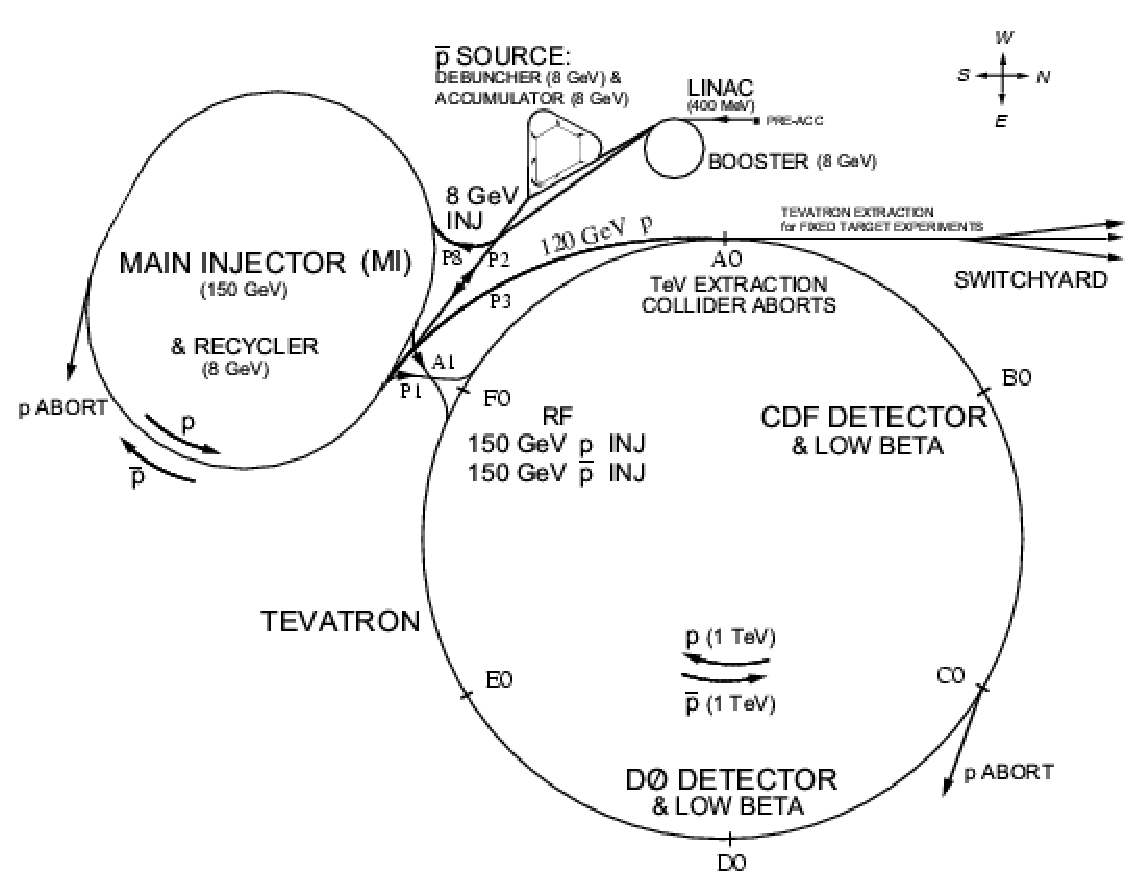
\includegraphics[width=6in,angle=0]{eps/Tevatron/Tevatron.eps}
\caption{Schematic of the Fermilab accelerator complex~\cite{Haas:2004rx}.}
\label{FermilabAccelerator}
\end{figure}

\subsection{Cockcroft-Walton}
The first accelerator in the chain is the Crockroft-Walton. In this accelerator a hydrogen gas is heated which allows an additional electron to bond with the hydrogen atom producing a net negative charge. The Crockroft-Walton is a DC voltage ladder that produces a voltage difference of 750~kV across which the newly negatively hydrogen ions are accelerated.

\subsection{LINAC}
After the negatively charged hydrogen ions have been accelerated to an energy of 750keV, they are further accelerated by the LINAC (LINear ACcelerator). The LINAC is a 130-m long set of metallic drift tubes separated by vacuum gaps. An alternating electric field produced by a radio frequency (RF) power source accelerates the negatively charged hydrogen ions across the gap while the electric field is parallel with the ion direction of motion. When the field direction reverses the ions are shielded by the metallic drift tubes. As the ions increase their speed the gap length and drift tube length increases as shown in Fig.~\ref{LINAC}. Because the LINAC uses an alternating electric field the continuous ion beam produced by the Crockoft-Walton is altered such that the protons are concentrated or ``bunched" together. By the end of the acceleration the proton bunches are separated by 5 ns and have an energy of 400 MeV. Finally, the orbital electrons are removed by passing the ions through a carbon foil leaving behind the positively charged protons.

\begin{figure}[!h!tbp]
\begin{center}
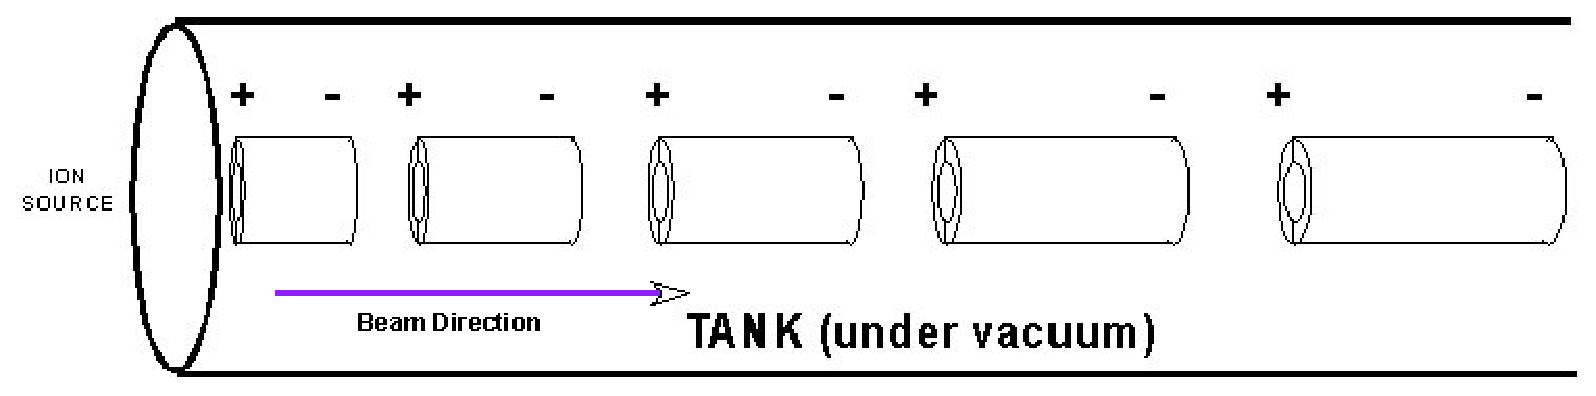
\includegraphics[width=0.75\textwidth]{eps/Tevatron/LINAC.eps}
\end{center}
\vspace{-0.1in}
\caption{Cartoon example of the linear accelerator's alternating series of gaps and drift tubes~\cite{proton}.}
\label{LINAC}
\end{figure}

\subsection{Booster}
The next accelerator in the chain is the Booster, which is a circular synchrotron accelerator 475-m in circumference. The Booster consists of RF cavities that accelerate the 400 MeV proton bunches to an energy of 8 GeV. The proton bunches circulate the Booster 16,000 times and the entire acceleration process takes 33 ms.

\subsection{Main Injector}
The Main Injector is the next accelerator in the chain after the Booster. This accelerator uses RF cavities to accelerate the proton bunches to an energy of 120 GeV and employs strong magnets to keep the protons moving along a circular path. After the acceleration there are two possible paths for the protons: $\bar{p}$~production or continued acceleration. The protons that will eventually circulate in the Tevatron ring are further accelerated to an energy of 150 GeV and then continue to circulate the Main Injector ring until needed~\cite{proton}. The remaining protons are used to create antiprotons that will also eventually circulate in the Tevatron ring. Antiprotons are created when 120 GeV protons from the Main Injector strike a fixed 7 cm thick nickel target producing a spray of short lived particles and anti-particles. From this spray roughly 20 antiprotons are produced for every million protons used~\cite{Antiproton}. All particles produced from the collision are focused and collimated by a lithium lens. A bending magnetic is employed to separate the negatively charged antiprotons from all positively charged particles. To remove the remnant bunch structure the antiprotons are passed through a debuncher, which separates the antiprotons in space-time as well as reducing their energy spread. A process known as stochastic cooling is applied to further reduce the energy spread. This process uses ultra-cold electronics (-$269^{\circ}$~C) to detect and alter the particles trajectories to make their orbits and thereby their energies more uniform. Because each $\ppbar$~collision requires $\sim10^{10}$ antiprotons the final stage for $\bar{p}$~production is to collect and store large quantities of antiprotons. This is done with the accumulator, which allows for many circulating beams of antiprotons to be kept for many hours. Once enough antiprotons have been collected they are sent to the Main Injector where they are accelerated to a final energy of 150 GeV.

\subsection{Tevatron}

The Tevatron is the final acceleration stage for the protons and antiprotons, which reach an energy of 980 GeV using RF cavities in the same manner as the Booster and the Main Injector~\cite{tevatron}. The Tevatron uses nearly 1,000 superconducting magnets running at $4.3^{\circ}$~K with a magnetic field strength of $4.2$~T to bend the two circulating beams around the nearly 6~$\frac{1}{2}$ km circumference ring. At an energy of 980 GeV the bunches circulate the Tevatron ring nearly 57,000 times per second crossing one-another every 396 ns. The two circulating beams are separated in the ring to avoid direct collisions unless they are further focused. In the Tevatron ring there are two places where the beams are focused, which correspond to the two large experiments: $\dzero$ and CDF.

\section{$\ppbar$~Collisions}
\label{ppbarcollisions}

When the two circulating beams at the Tevatron are brought into focus, an enormous range of kinematically allowed processes and final state decays are possible. While the outcome of a particular $\ppbar$~collision is random, the rate at which certain processes occur can be calculated within the Standard Model framework. The most common type of collision is an inelastic $\ppbar$~collision which produces one or more particles scattered at low angles with respect to the beam axis. These processes usually do not involve much energy transfer between the colliding particles and are therefore called low-$p_{T}$ events. More rare processes, such as top quark or $W$ boson production, require much more energy to be transferred between colliding particles. These processes occur when one of the constituent quarks or gluons inside the proton collide with another quark or gluon from the antiproton. This process is referred to as the hard scatter process. The hard scatter process can produce on-shell resonances ($Q^{2} = M^{2}$) of heavy particles such as a $W$ Boson or sometimes it can produce very short lived vritual particles ($Q^{2} \neq M^{2}$) such as the case with $s$-channel single top quark production where a $W$ boson is produced with $Q^{2} > M_{W}^{2}$.

The heavy particles produced in the hard scatter collision will decay into more stable particles as governed by the interactions allowed in the Standard Model. For very heavy particles with short lifetimes the decay occurs in a space much smaller than the resolution of any detector. For instance, the top quark lifetime is $\sim10^{-24}$~s which is more than nine orders of magnitude smaller than the fastest detector electronics. In fact almost all short-lived particles produced in the hard scatter can not be measured directly, but instead their presence is inferred from precise measurements of the their decay products.

The remainder of this chapter is dedicated to describing the $\dzero$~detector and how it makes the measurements required to infer the presence of heavy resonances such as the top quark. Section~\ref{coordinate} gives a short introduction to the coordinate system convention used throughout the rest of the chapter as well as introduces several new units typically used in high energy physics. Section~\ref{detector} describes the $\dzero$~detector and explains how it is used to measure the particles resulting from the $\ppbar$~collisions at the Tevatron.

\section{Coordinate System and Units Convention}
\label{coordinate}

The $\dzero$~detector is typically referenced using a spherical coordinate system ($r$,$\theta$,$\phi$) with an origin located at the center of the detector. The polar angle $\theta$ is defined with respect to the beam axis where $0^{\circ}$ is aligned with the proton direction and $180^{\circ}$ is aligned with the antiproton direction. The azimuthal angle $\phi$ is defined with respect to the $x$-axis as shown in Fig.~\ref{coordinate-eps}. The $z$-axis is defined to be parallel with the beam axis with the positive direction corresponding to $\theta = 0^{\circ}$ and the negative direction corresponding to $\theta = 180^{\circ}$.

\begin{figure}[!h!tbp]
\begin{center}
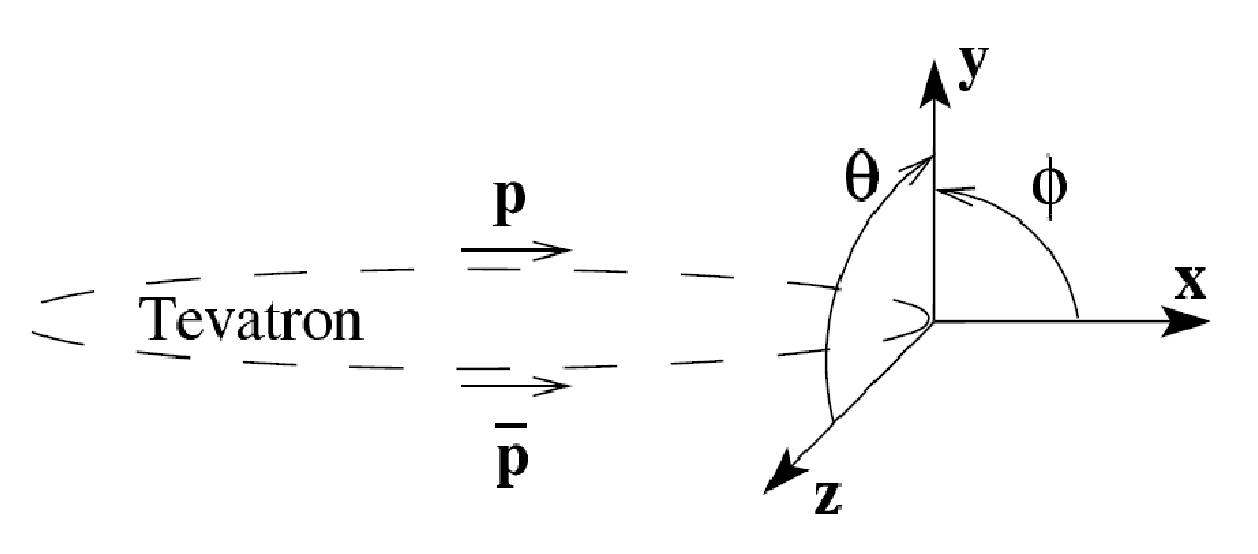
\includegraphics[width=0.75\textwidth]{eps/Tevatron/Coordinate.eps}
\end{center}
\vspace{-0.1in}
\caption{$\dzero$ coordinate system with respect to the Tevatron ring~\cite{Stelzer:2005kz}.}
\label{coordinate-eps}
\end{figure}

It often convenient to convert the angle $\theta$ to a quantity called pseudorapidity $\eta$ defined in Eq.~\ref{pseudorapidity}.

\begin{equation}
\label{pseudorapidity}
\eta = -\ln \left[ \tan \left( \frac{\theta}{2} \right) \right]
\end{equation}

This quantity is identical, in the limit of massless particles, to the true rapidity $y$, shown in Eq.~\ref{rapidity}, which is invariant under a Lorentz boost along the $z$-direction. This is useful because $\ppbar$~collisions at the Tevatron usually occur with such a boost. The pseudorapidity is $0$ for a particle with $\theta = 90^{\circ}$ and approaches $\infty$ as $\theta \rightarrow 0^{\circ}$.

\begin{equation}
\label{rapidity}
y = \frac{1}{2}\log \left[ \frac{E + p_{z}}{E - p_{z}} \right]
\end{equation}

Another quantity used when describing the relationship between two objects or the size of an object in the $\dzero$~detector is the solid angle $\Delta R$ defined in terms of $\Delta\phi=\phi_{1} - \phi_{2}$~and $\Delta\eta=\eta_{1} - \eta_{2}$.

\begin{equation}
\Delta R = \sqrt{(\Delta\phi)^{2} + (\Delta\eta)^{2}}
\end{equation}

Finally, the luminosity is important when describing the intensity of an interaction or of the accumulated amount of data. The rate of a certain process is equal to the luminosity $\mathcal{L}$ times the Lorentz invariant cross section $\sigma$, as shown in Eq.~\ref{rate}.

\begin{equation}
\label{rate}
\rm{Rate} = \frac{dN}{dt} = \sigma * \mathcal{L}
\end{equation}

Most cross sections at the Tevatron are given in terms of pico-barns ($10^{-36}$~cm$^{2}$) thus the units of luminosity are pb$^{-1}$s$^{-1}$. The time integrated luminosity $\int \mathcal{L} dt$, with units of pb$^{-1}$, is used when discussing the total number of collected events.

\section{\dzero~ Detector}
\label{detector}

The $\dzero$~detector~\cite{Abazov:2005pn} is a collection of smaller sub-detectors working in tandem  to detect and measure all particles produced from the hard scatter collision. The inner-most detectors near the beam pipe are the tracking detectors, described in Section~\ref{tracking}, which record the paths of charged particles as they enter and leave the detector. The next layer of the detector is the calorimeter, described in Section~\ref{calorimetry}. The calorimeter measures the energy of the lightest electromagnetically interacting particles, such as the electron and the photon, and strongly interacting particles, such as pions or neutrons. Another sub-detector, called the luminosity monitor, described in Section~\ref{luminositydetector}, is designed to record the presence of an inelastic $\ppbar$~collision in the bunch crossing. This information is used in the analysis to normalize backgrounds and expected signal yields. The outer-most layer of the $\dzero$~detector is the muon detector, which is described in Section~\ref{muondetector}. Once the collision has been measured a complex set of trigger decisions, described in Section~\ref{triggersystem}, must be satisfied before the event is recorded to tape for later analysis.

\begin{figure}[!h!tbp]
\begin{center}
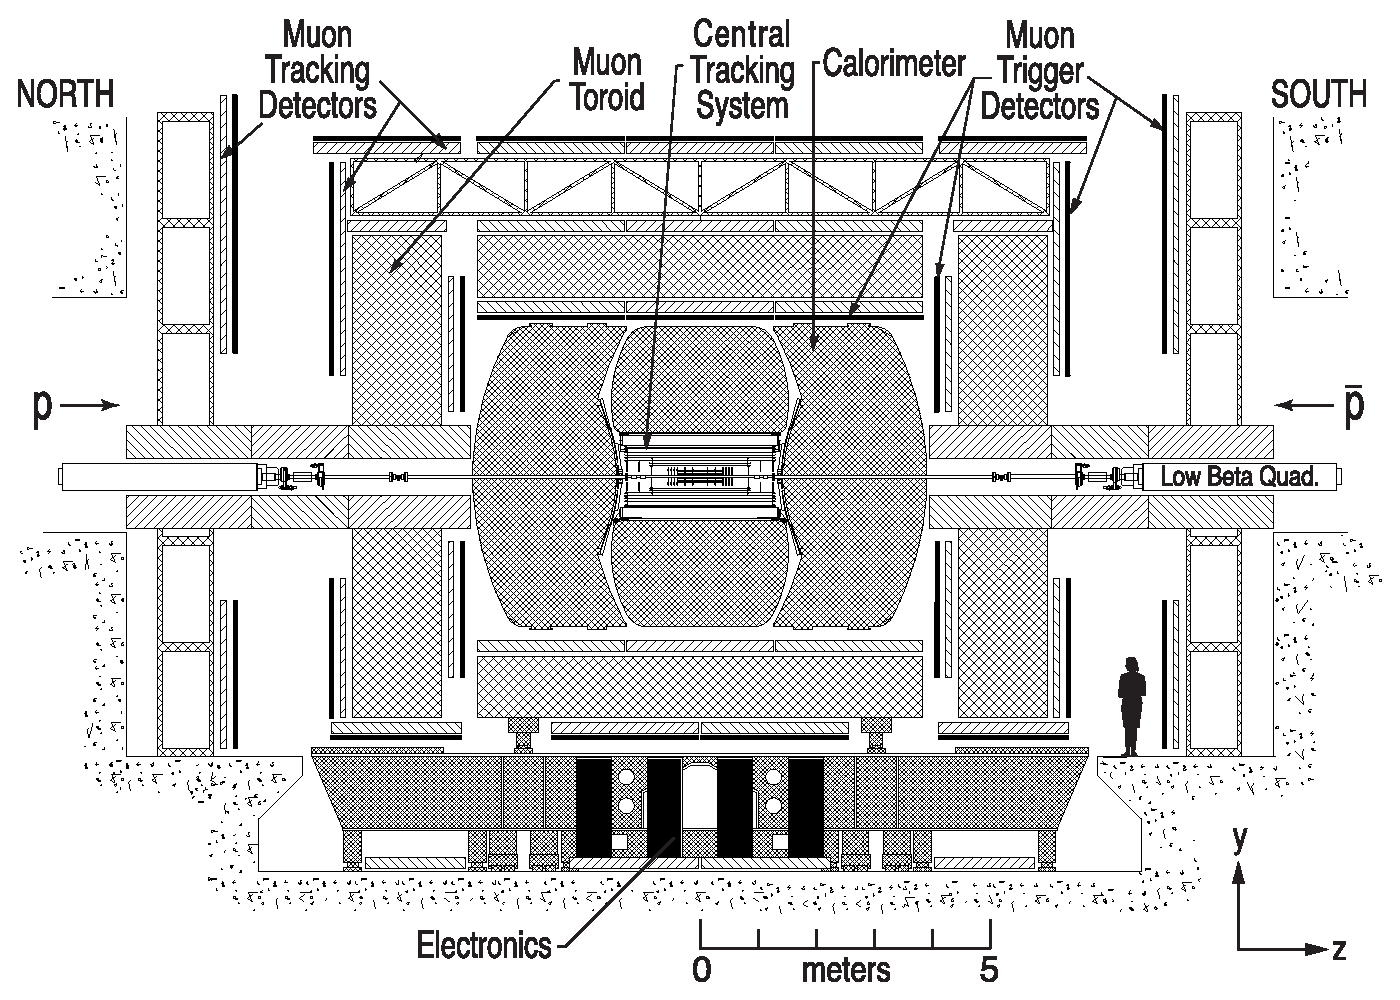
\includegraphics[width=1.0\textwidth]{eps/D0/DetectorSlice.eps}
\end{center}
\vspace{-0.1in}
\caption{Schematic side-view of the $\dzero$~detector~\cite{Abazov:2005pn}.}
\label{D0}
\end{figure}

\subsection{Tracking Detectors}
\label{tracking}

The innermost layer of the $\dzero$~detector is a set of two tracking detectors designed to measure the flight path of charged particles. The two detectors, shown in Fig.~\ref{InnerDetector}, are the silicon microstrip tracker (SMT) and the central fiber tracker (CFT). The SMT and CFT are located within a 2T magnetic field generated by a superconducting solenoid magnet. The presence of the magnetic field within the tracking detectors will deflect all charged particles allowing a measure of the their charge and momentum through the sign and radius of the induced curvature.

\begin{figure}[!h!tbp]
\begin{center}
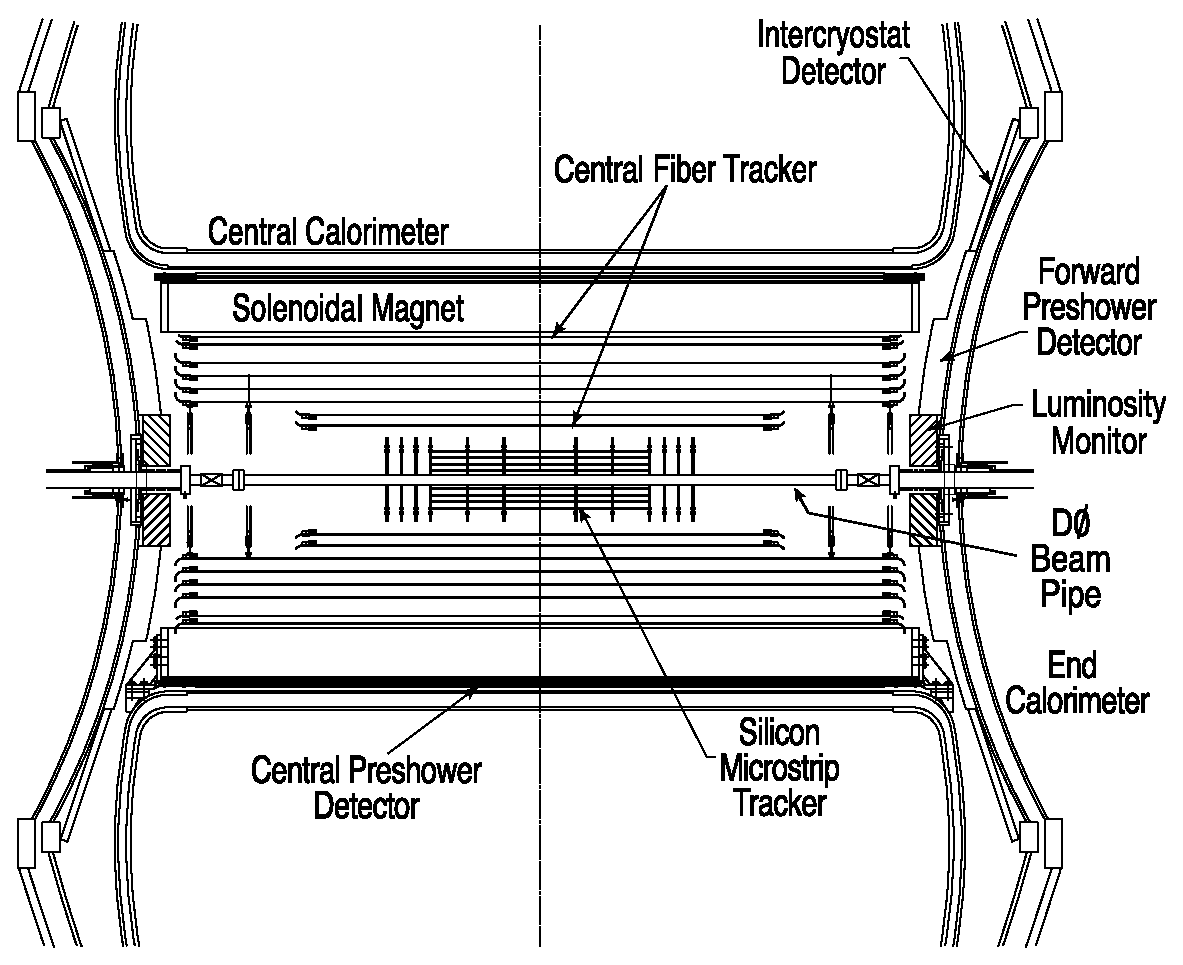
\includegraphics[width=0.75\textwidth]{eps/D0/InnerDetector.eps}
\end{center}
\vspace{-0.1in}
\caption{Schematic of the two tracking detectors (SMT and CFT) as well as the superconducting solenoid magnet~\cite{Abazov:2005pn}.}
\label{InnerDetector}
\end{figure}

\subsubsection{Silicon Microstrip Tracker}

The SMT is located immediately outside the Tevatron beam pipe and is designed to provide high resolution position measurements of charged particles. The SMT is a collection of doped silicon detectors depleted of electric charge by the application of a reverse bias voltage. As a charged particle enters the depleted region it ionizes the silicon creating electron-hole pairs. The result of the applied electric field is to force the charges to drift towards active sensors. The typical drift distance for charges in the silicon is $300$~$\mu$m. A schematic of the SMT is shown in Fig.~\ref{SMT}.

\begin{figure}[!h!tbp]
\begin{center}
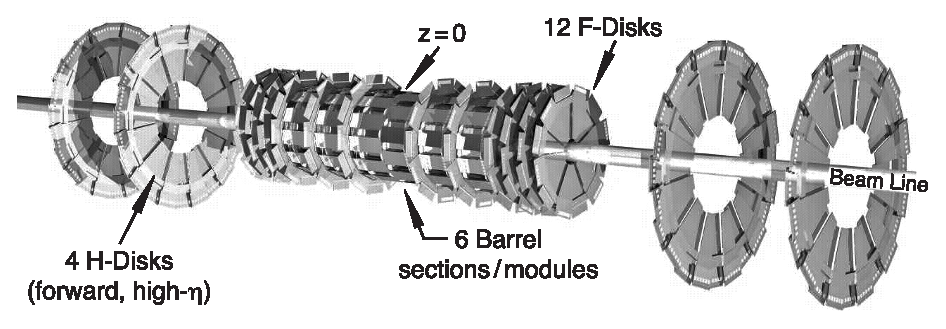
\includegraphics[width=0.75\textwidth]{eps/D0/SMT.eps}
\end{center}
\vspace{-0.1in}
\caption{Schematic of the silicon microstrip tracker sub-detector~\cite{Abazov:2005pn}.}
\label{SMT}
\end{figure}

The geometry of the SMT is dictated by the length of the interaction region\footnote{The typical Gaussian width of the hard scatter interactions is $25$~cm centered around z=0.} and a desire to maximize the number of layers a charge particle traverses. To achieve this goal the detector is organized into three structures: the barrel detector, the F-discs, and the H-discs. The barrel detector is a set of six barrels concentric with the beam pipe that each contain four double-sided layers of silicon wafers. The barrels provide coverage for centrally produced charged particles with $|\eta|<1.1$. The F-discs are also double-sided silicon wafers. These silicon detectors are oriented perpendicular to the beam axis in contrast with the concentric barrels. There are twelve F-disks in the SMT, six in the central region that cap each barrel and six in the forward region. The SMT also has four silicon detectors at high $|z|$ called H-disks, which are oriented perpendicular to the beam axis. In total the SMT has 912 individual readout modules and nearly 800,000 individual readout channels.


\subsubsection{Central Fiber Tracker}

Immediately outside of the SMT is the central fiber tracker (CFT) which occupies the radial distance of 20 to 52 cm from the beam pipe. The CFT is organized into 8 layers of scintillating fibers which produce light when a charged particle traverses the fibers. Each layer of the CFT consists of two sets of fibers: one that is parallel with the beam axis and one that is rotated $3^{\circ}$ with respect to the beam axis. 
The fibers in the tracker are $835$~$\mu$m in diameter and composed of organic scintillating compounds surrounded by a thin layer of cladding designed to provide total internal reflection inside the fiber. The light produced in the fiber is carried out of the detector by wave guides with typical travel distances between 8 and 11 m. Because the light is only read out at one end of the fiber the other end is coated with sputtered aluminum which reflects 90$\%$ of the light back to the end which is read out. An endview schematic of the CFT layers and their associated waveguides is shown in Fig.~\ref{CFT}.  Light produced in the CFT is recorded on silicon avalanche photon counters called VLPCs (visible light photon counter). The VLPCs operate at $9^{\circ}$~K to reduce thermal noise and achieve a quantum efficiency of $75\%$.

\begin{figure}[!h!tbp]
\begin{center}
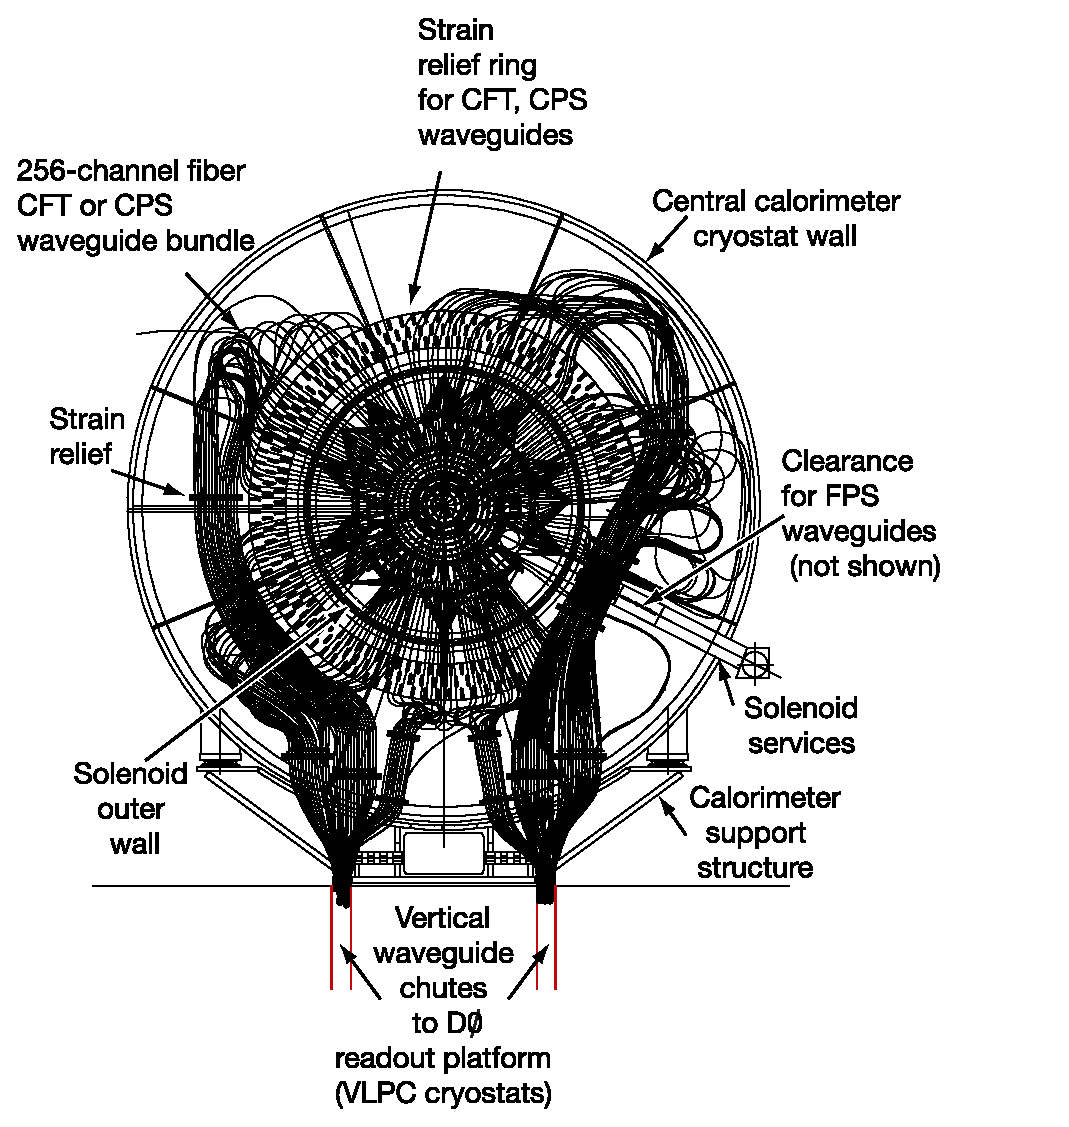
\includegraphics[width=0.75\textwidth]{eps/D0/CFT.eps}
\end{center}
\vspace{-0.1in}
\caption{Schematic endview of the central fiber tracker with corresponding waveguides~\cite{Abazov:2005pn}.}
\label{CFT}
\end{figure}

\subsection{Calorimetry}
\label{calorimetry}

The next layer of the $\dzero$~detector is the calorimeter. The calorimeter is designed to measure the energy of electromagnetically interacting particles such as electrons and photons as well as strongly interacting particles such as pions and neutrons. The $\dzero$~calorimeter is divided into three sub-detectors: one central region (CC) and two end-cap regions (EC) as seen in Fig.~\ref{Calorimeter}. Each region is encased in its own cryostat held at a constant temperature of $90^{\circ}$~K. The region between the two cryostats, $0.8 < |\eta| < 1.4$, is called the inner cryostat region (ICR) and contains active scintillator to provide a minimal energy measurement in this region.

\begin{figure}[!h!tbp]
\begin{center}
\includegraphics[width=0.75\textwidth]{eps/D0/Calorimeter.eps}
\end{center}
\vspace{-0.1in}
\caption{3D view of the $\dzero$ calorimeter~\cite{Abazov:2005pn}.}
\label{Calorimeter}
\end{figure}

Each detector region, except the ICR, measures energy using a similar approach by inducing the incoming particles to produce an electromagnetic shower as they collide with a dense material. As particles from the shower enter the active region they will ionize the material. The ions in the active material move towards a sensor due to an applied bias voltage. The amount of charge collected on the sensor is then proportional to the energy deposited by the ionizing particle. An example of an electromagnetic shower originating from a photon is shown in Fig.~\ref{EMshower}.  The typical ion drift time in the $\dzero$~calorimeter is $\sim450$~ns.


\begin{figure}[!h!tbp]
\begin{center}
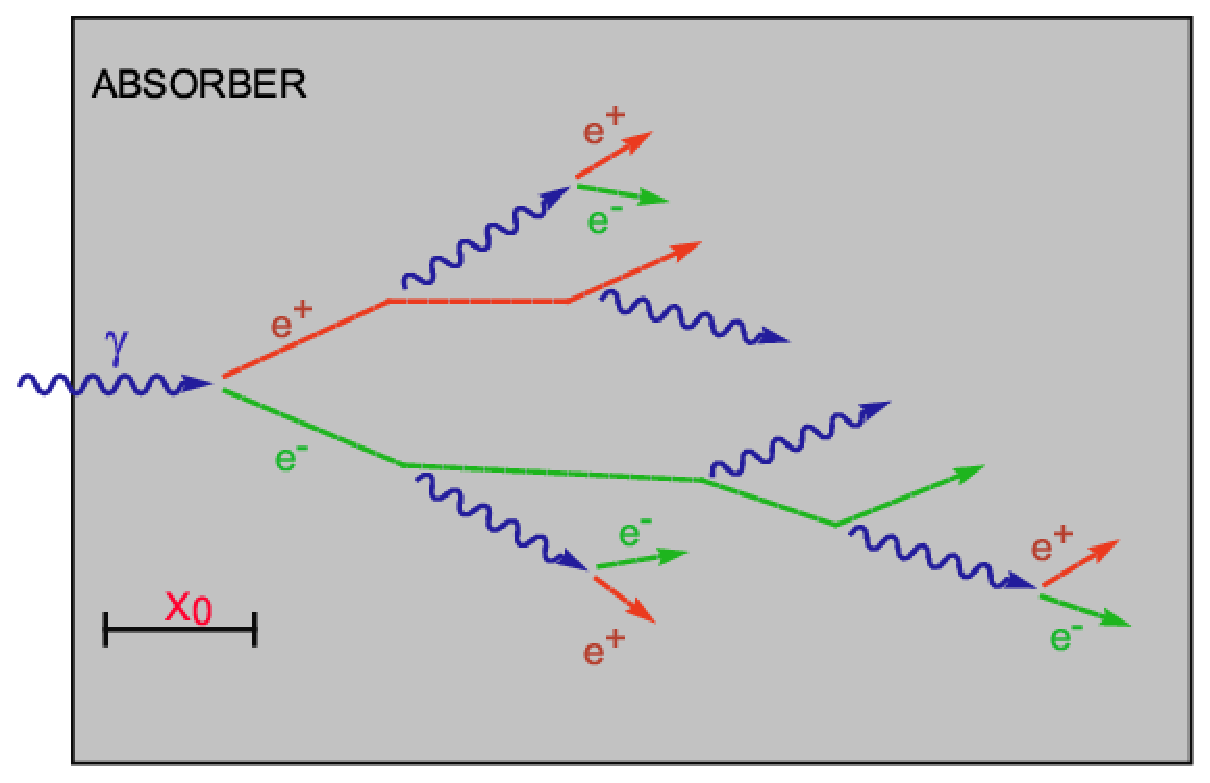
\includegraphics[width=0.75\textwidth]{eps/D0/shower.eps}
\end{center}
\vspace{-0.1in}
\caption{Initial stages of an electromagnetic shower caused by a photon interacting with an absorber material. The radiation length $x_{0}$ is the typical distance a photon will travel before producing an $e^{+}e^{-}$ pair or the distance before an electron will radiate a photon~\cite{shower}.}
\label{EMshower}
\end{figure}

The $\dzero$ calorimeter consists of an inner detector called the EM calorimeter and an outer detector called the hadronic calorimeter. The EM calorimeter is constructed of alternating layers of depleted Uranium, which acts as the shower inducing material, and liquid Argon, which acts as the active medium. The depleted Uranium plates are 3 mm thick in the central region and 4 mm thick in the forward end-cap region while the liquid Argon active region is 2.3 mm thick. An cartoon drawing of this arrangement can been seen in Fig.~\ref{CalorimeterCell}. The EM calorimeter has four layers of cells representing nearly 21 radiation lengths. The hadronic calorimeter is actually two detectors: one called the fine hadronic calorimeter which employs 6 mm thick Ur-Ni alloy as the shower inducing material and the coarse hadronic calorimeter which uses 46.5 mm thick plates of copper in the central region and stainless steel in the forward region. The hadronic calorimeter also uses liquid Argon as the active material. The combination of the fine and coarse hadronic calorimeters provides an additional 7 radiation lengths to the detector. The numerous radiation lengths are important to ensure that a particle deposits nearly all of its energy in the detector.


\begin{figure}[!h!tbp]
\begin{center}
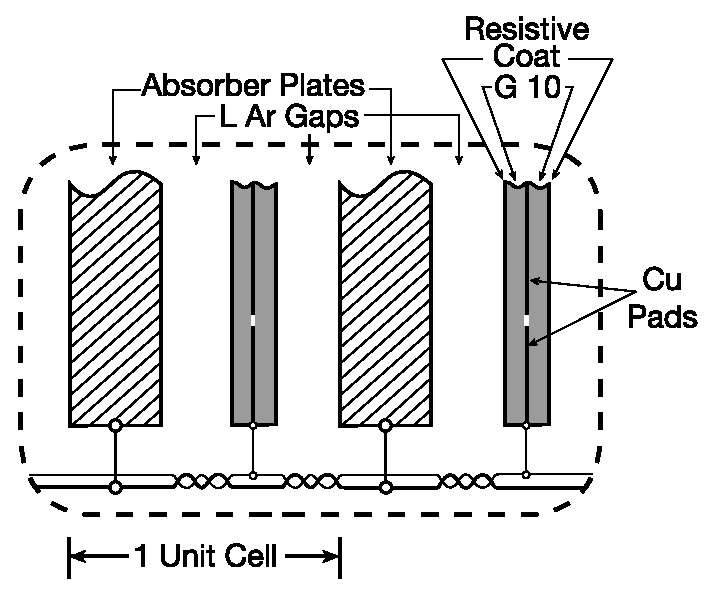
\includegraphics[width=0.75\textwidth]{eps/D0/CalorimeterCell.eps}
\end{center}
\vspace{-0.1in}
\caption{Example of a typical calorimeter cell of alternating absorber and active material. Particles traverse the calorimeter cell from left to right in this diagram~\cite{Abazov:2005pn}.}
\label{CalorimeterCell}
\end{figure}

The $\dzero$~calorimeter also has fine segmentation (i.e. radial size of the cells), which allows for excellent energy and position measurement of particles as they shower in the detector. The segmentation of the EM calorimeter in $\delta\eta \times \delta\phi$ is $0.1 \times 0.1$ for all layers except the third layer, where the segmentation is $0.05 \times 0.05$. The fine segmentation in the third layer 
is because the electromagnetic shower is expected to reach a maximum in this layer. The fine hadronic layers of the calorimeter also have a segmentation of $0.1 \times 0.1$, while the segmentation in the coarse hadronic calorimeter is $0.2 \times 0.2$. An octant of the $\dzero$~calorimeter including segmentation can be seen in Fig.~\ref{CalorimeterSegmentation}. 

\begin{figure}[!h!tbp]
\begin{center}
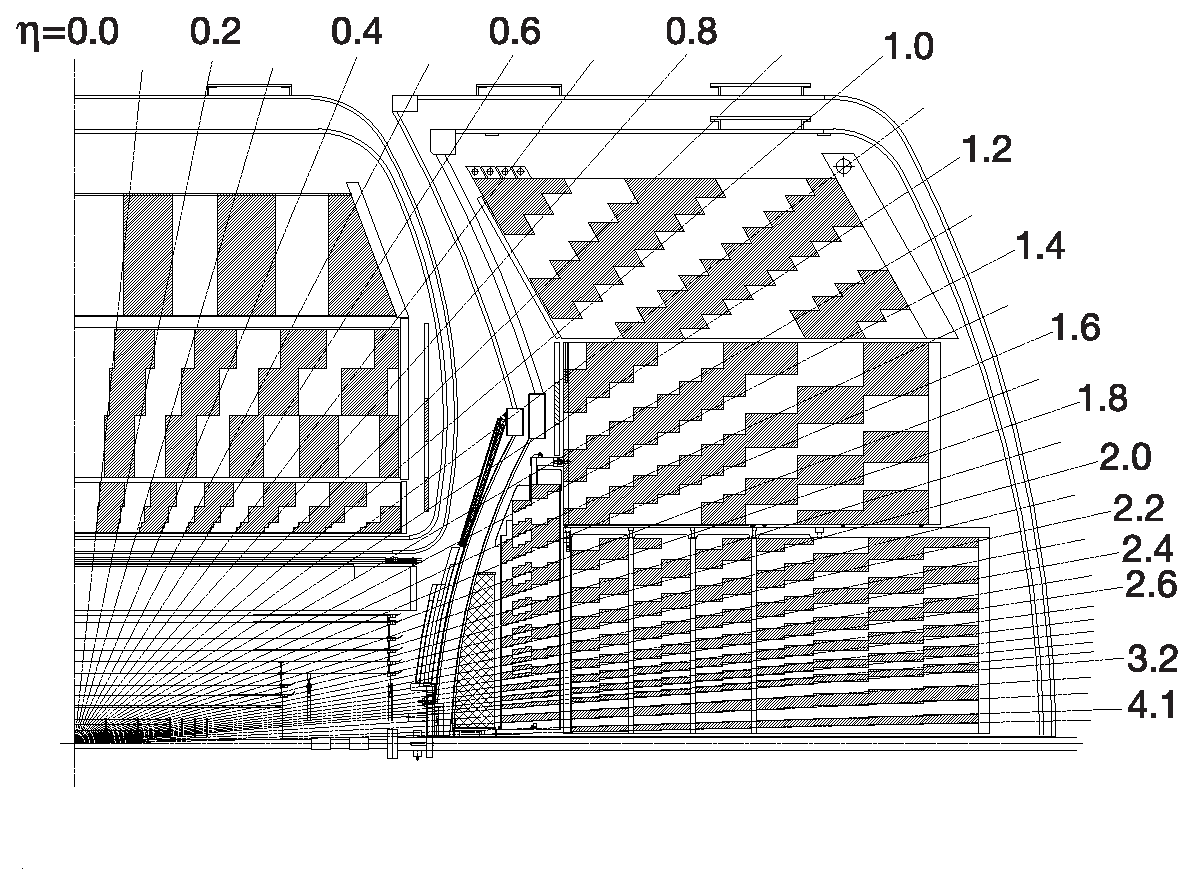
\includegraphics[width=0.75\textwidth]{eps/D0/CalorimeterSegmentation.eps}
\end{center}
\vspace{-0.1in}
\caption{Octant of the $\dzero$~calorimeter. The fine segmentation of the calorimeter is clearly seen in this diagram~\cite{Abazov:2005pn}. The alternating dark and light blocks represent cells in different calorimeter towers.}
\label{CalorimeterSegmentation}
\end{figure}



\subsection{Luminosity Monitor}
\label{luminositydetector}

Located directly in front of the end-cap calorimeters, covering a $\eta$ range between 2.7 and 4.4, is the luminosity monitor, which collects information about inelastic $\ppbar$~collisions for each bunch crossing. The luminosity monitor is a set of 24 plastic scintillators which can detect low angle (high $\eta$) fragments from the break-up of the protons in the $\ppbar$~collision. The scintillators produce light when the charged fragments traverse the detector and that light is recorded by photo-multiplier tubes. A schematic of the luminosity monitor is shown in Fig.~\ref{Luminosity}.

\begin{figure}[!h!tbp]
\begin{center}
\includegraphics[width=0.75\textwidth]{eps/D0/Luminosity.eps}
\end{center}
\vspace{-0.1in}
\caption{Schematic of the $\dzero$ luminosity monitor shown in relation to the beam pipe, SMT, and endcap calorimeter~\cite{Abazov:2005pn}.}
\label{Luminosity}
\end{figure}


Collecting information about inelastic collisions is vital to properly normalize all data collected at $\dzero$. The luminosity monitor is designed to measure the inelastic $\ppbar$~cross section, which is a quantity that is known from measurements by previous experiments. By measuring the inelastic $\ppbar$~cross section the total integrated luminosity to which the $\dzero$~detector has been exposed to can be measured~\cite{d0note4958,d0note5139}. A derivation of the luminosity from the measured $\ppbar$~inelastic cross section can be found in Appendix~\ref{lumi}.

Along with providing a luminosity measurement, the detector also acts as a fast vertex finder. By measuring the relative difference of coincidence counts in the North and South detectors the $z$ position of the vertex can be determined from Eq.~\ref{zpos}, where $t_{\pm}$ are the time measured by the North (+) and South (-) detectors, respectively. The time of flight resolution for the luminosity detector is 0.3 ns.

\begin{equation}
\label{zpos}
z = \frac{c}{2}(t_{+} - t_{-})
\end{equation}

\subsection{Muon Detector}
\label{muondetector}

The outer-most layer of the $\dzero$~detector is the muon system. A special detector is required to measure muons because they do not deposit much energy in the tracker or calorimeter and thus a confirmation of their presence using these sub-detectors alone is difficult to infer. The muon detector has two active regions called the central region for $|\eta|<1$ and the forward region for $1<|\eta|<2$. The system also employs a 2 T toroid iron magnet to bend the muons from their original paths. The addition of the magnetic field helps to provide a local momentum measurement in the event the momentum can not be determined from the tracking detector. Additional shielding surrounding the beam pipe near the forward muon detector is designed to reduce spurious beam effects which dramatically reduces the amount of radiation to which to detector is exposed. A schematic of the muon system and the beam shielding can be seen in Fig.~\ref{MuonDetector}.

\begin{figure}[!h!tbp]
\begin{center}
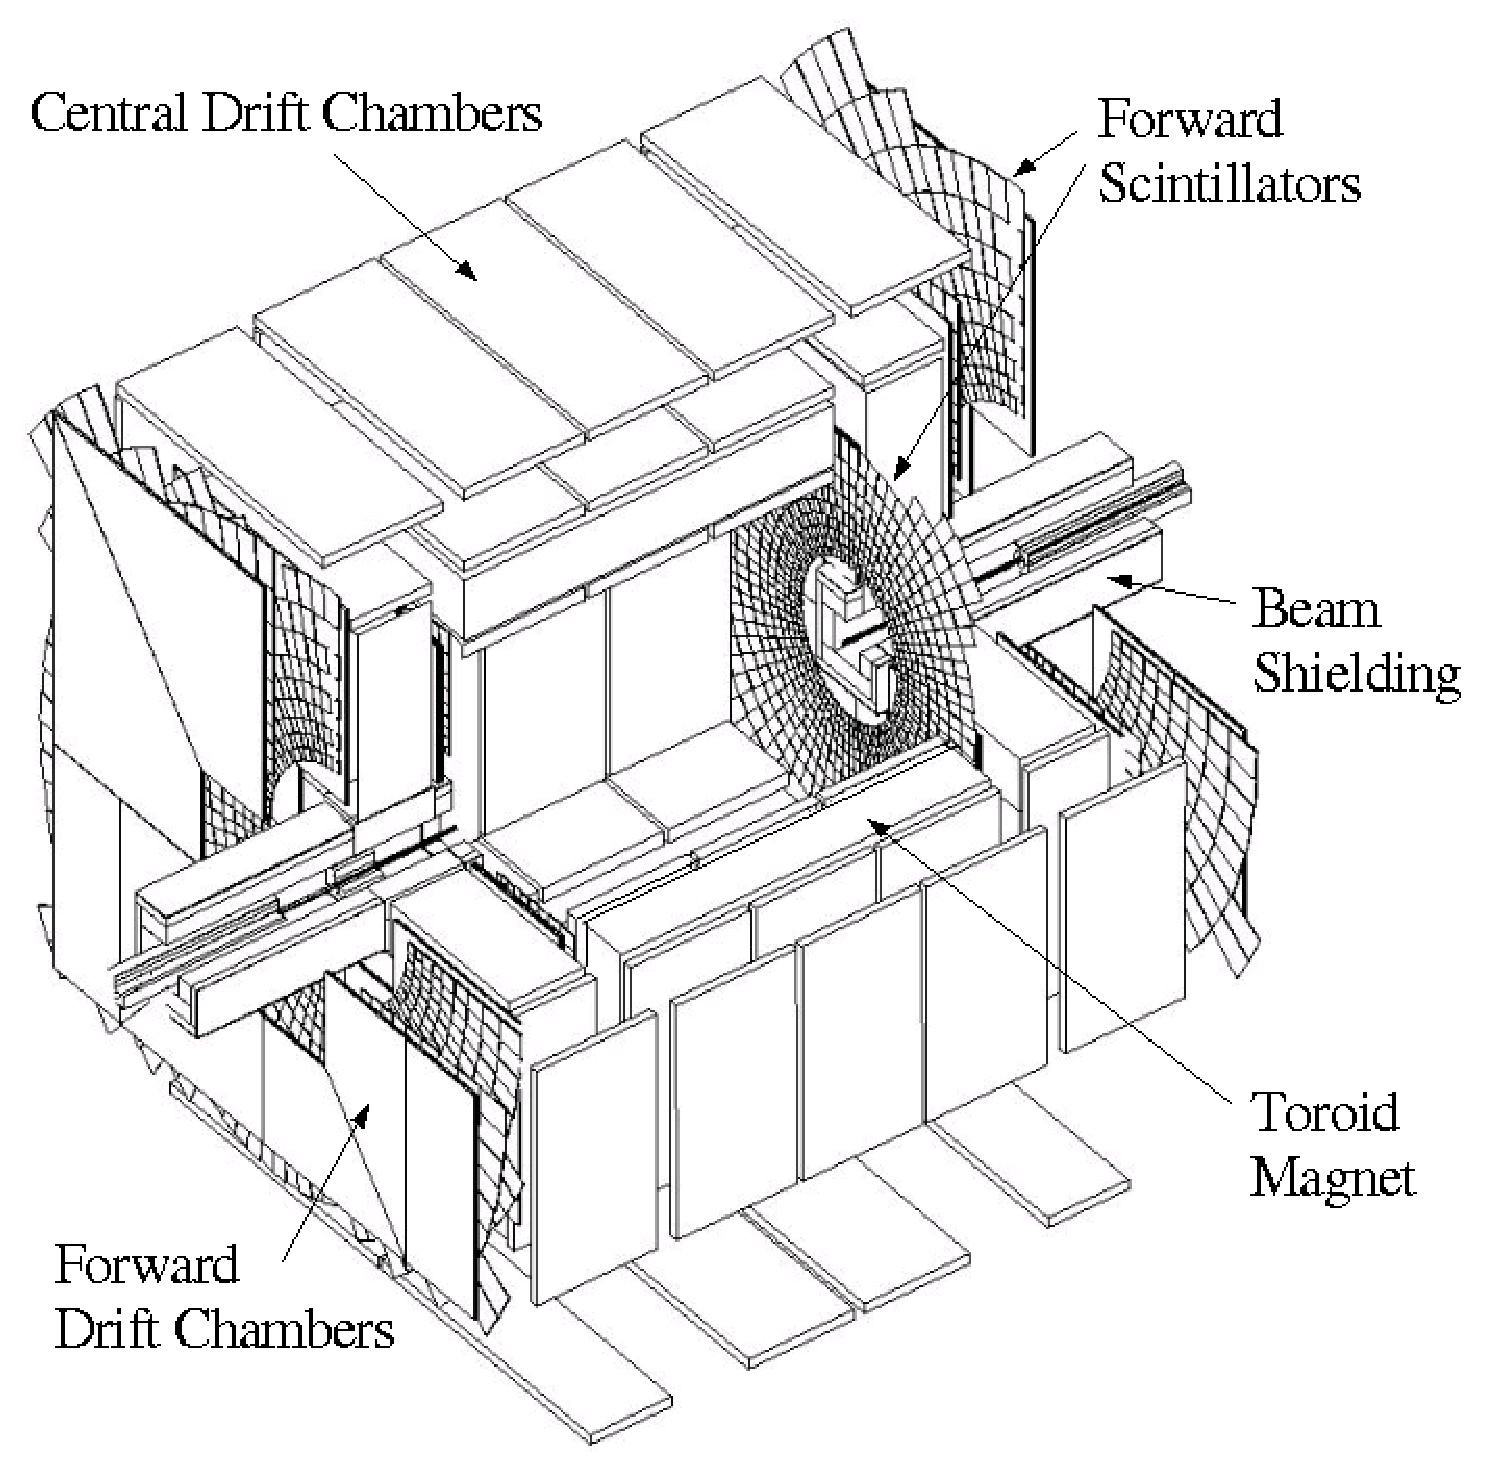
\includegraphics[width=0.75\textwidth]{eps/D0/mudet.eps}
\end{center}
\vspace{-0.1in}
\caption{3D view of the $\dzero$ muon detector~\cite{Abazov:2005pn}.}
\label{MuonDetector}
\end{figure}

The muon system at $\dzero$ is a three layer detector, both in the central and forward regions, consisting of drift chambers for precise position measurement and scintillator counters for muon identification and fast triggering (Section~\ref{triggersystem}). The scintillator counters produce light when the muon passes through the detector which is then collected by a photo-multiplier tube. The drift chambers have a central wire held at a large voltage surrounded by an inert gas. As the muon enters the chamber it will ionize the gaseous organic compound mixture and the resulting free charges will drift towards the wire. The position of the muon is found by analyzing the current profile in the wire. In the central region the drift chambers are called PDTs (proportional drift tubes) and are rather large with typical areas of 2.8 $\times$ 5.6 m$^{2}$. The forward region uses smaller drift chambers called MDTs (mimi drift tubes), which are a collection of eight cells of size 9.4 $\times$ 9.4 mm$^{2}$. The position resolution of the drift chambers is $\sim$1 mm.

\subsection{Trigger and Data Acquisition System}
\label{triggersystem}

The previous sections in this chapter describe how the $\dzero$~detector collects information from $\ppbar$~collisions at the Tevatron, which occur every $396$~ns. While $\dzero$ records information about every collision, it does not save every event to tape for two reasons: most collisions at the Tevatron are small angle inelastic collisions which have already been well studied and the total rate of data one can reliably store to tape is limited to $\sim$30MB/s. Because $\dzero$~can not save every event, a sophisticated trigger system is employed to reduce the total rate to tape to $50$~Hz. This trigger system attempts to select the most ``interesting" events, which will be used for an analysis or future calibration of the detector.

The trigger system is comprised of three independent stages called level 1, level 2, and Level 3, which are designed to reduce the total event rate from $1.7$~MHz to $50$~Hz. A schematic of the combined trigger system is shown in Fig.~\ref{Trigger}. The level 1 system is composed of hardware trigger elements and has the goal of reducing the initial rate of  $1.7$~MHz to $1.5$~kHz. Because the level 1 trigger must act quickly to either accept or reject an event, the tools available for selecting interesting events is limited. At level 1 only calorimeter trigger towers, which are layers of calorimter cell energies within a $\delta\eta \times \delta\phi = 0.2 \times 0.2$ space, signals in the muon drift chambers or scintillators, and the transverse momentum of charged particle tracks in the central fiber tracker are available for trigger decisions.

\begin{figure}[!h!tbp]
\begin{center}
\includegraphics[width=0.75\textwidth]{eps/D0/TriggerFlow.eps}
\end{center}
\vspace{-0.1in}
\caption{Cartoon drawing of the $\dzero$ trigger system~\cite{Abazov:2005pn}.}
\label{Trigger}
\end{figure}

The level 2 trigger acts on all events which pass the level 1 trigger and is designed to reduce the rate from 1.5kHz to $700$Hz. The level 2 trigger uses detector specific pre-processing boards and a global detector board to make trigger decisions. The pre-processors collect data from the level 1 trigger system as well as readout information from the individual detectors. The pre-processors use this information to form physics objects such as electrons, jets, and missing E$_{T}$\footnote{Physics objects and event-wide kinematic variables such as missing E$_{T}$~are fully described in Chapter~\ref{EventSelection}.}. A global level 2 pre-processor uses all the information from the sub-detector pre-processors to make trigger decisions based on event-wide kinematics.

The next stage in the trigger selection process is the level 3 trigger, which is a software-based collection of algorithms executed on a collection of computer farm nodes. The goal of the level 3 trigger is to reduce the data rate to tape from $700$~Hz to $50$~Hz. The level 3 trigger requires the full detector readout to select events, thus all sub-detector data must be transmitted to the farm nodes. A level 3 data acquisition system was designed to transmit data over ethernet cables to the farm nodes. Upon a level 2 trigger accept a controller card in the sub-detector VME crate signals to a single board computer\footnote{The single board computers used in this DAQ are VMIC 7750 with a 933 MHz Pentium-III processor, 128 MB of RAM, 128  MB of on-board flash memory, and two 100 MB/s ethernet connectors. A few of the CFT crates use 2-1GB/s ethernet connector due to the high event sizes for these crates.}, located in the VME crate, to begin collecting the crate data and store it in RAM memory located on the SBC. While the data is being collected by the SBCs, a dedicated SBC called the Routing Master is collecting information about the event number as well as the level 1 and level 2 triggers that initially selected the event. The Routing Master communicates with the level 3 computer farm regarding its availability (i.e. if it is busy processing events or waiting for a new event) and assigns each event a unique farm node to which all SBCs must send the event information. This process is repeated for each event which is selected by the level 2 trigger. When the SBC has the full crate data stored in memory and a routing command issued by the Routing Master, the crate data is transmitted via one of two $100$~MB/s ethernet cables to the farm nodes.

Each event that is selected by the level 2 trigger ranges in size from 250 to 300~kB resulting in 200-300 MB/s of data being sent to the farm nodes. To handle this enormous data transfer rate, a set of CISCO 2948G ethernet switches concentrate ten 100~MB/s connections into a 1 GB/s optical fiber. The GB fibers are then brought to a CISCO 6509 ethernet switch capable of transmitting data at a rate of 16 GB/s. A schematic of this hardware setup and the data flow are shown in Fig.~\ref{l3all}.

\begin{figure}[!h!tbp]
\begin{center}
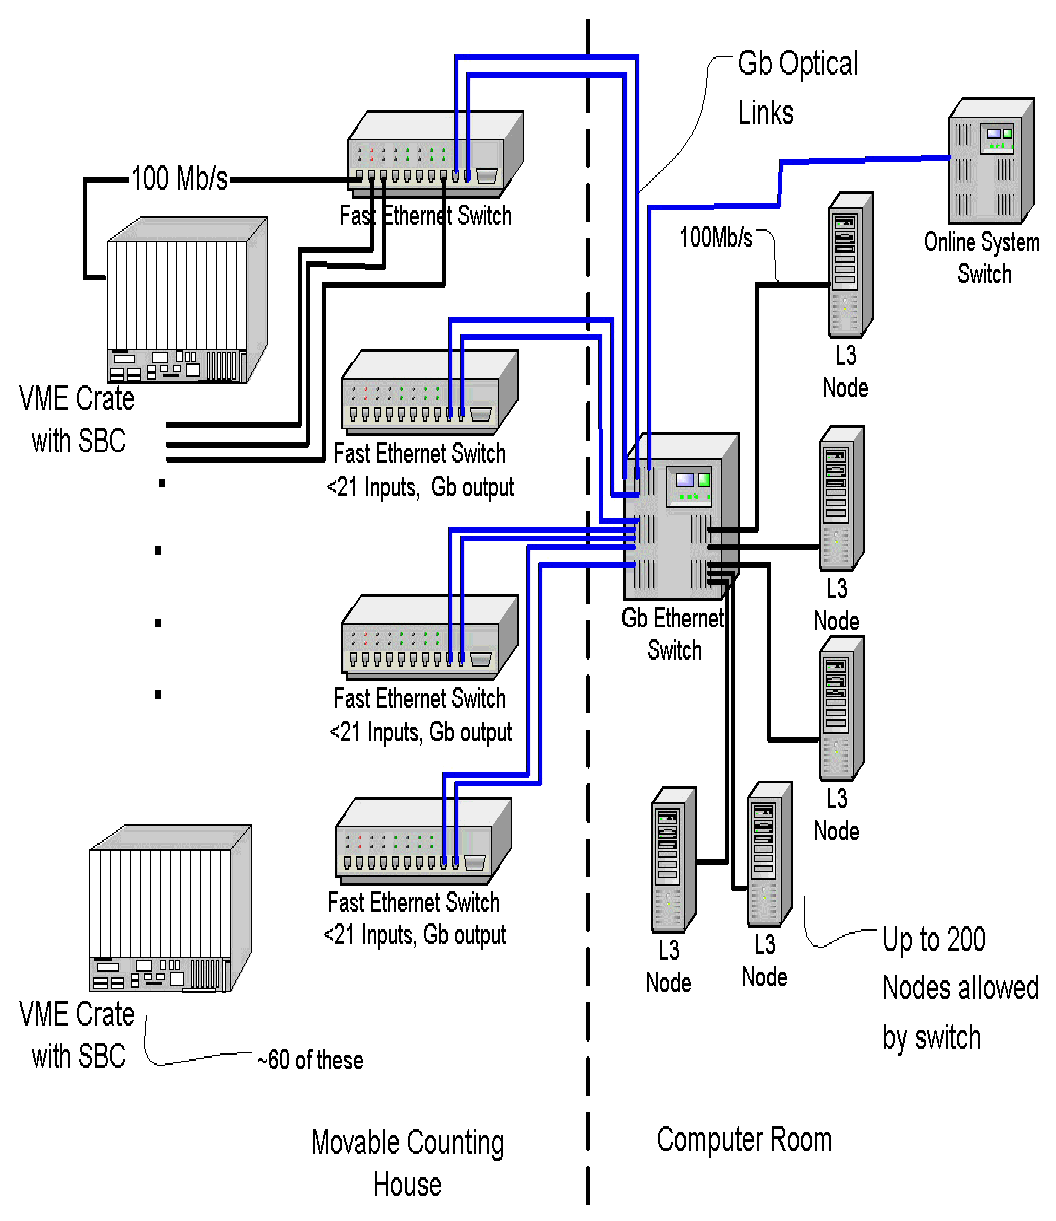
\includegraphics[width=0.49\textwidth]{eps/Level3/L3-DAQ.eps}
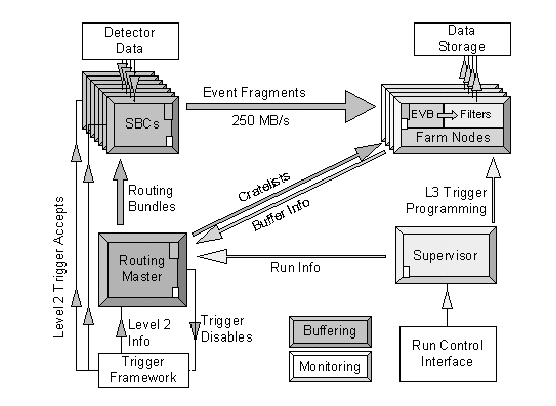
\includegraphics[width=0.49\textwidth]{eps/Level3/daq_software.eps}
\vspace{-0.1in}
\caption{Experimental setup of the level 3 trigger and data acquisition system (left) and the flow of data through the system (right).}
\label{l3all}
\end{center}
\end{figure}

When the data arrives at a farm node it is processed by a programmed called the Event Builder. This software package combines event fragments from each sub-detector data and organizes them into a readable format for the level 3 trigger software. If the Event Builder does not receive data from all sub-detector crates within a one second window after receiving the first fragment the event is dropped. As stated earlier the Event Builder transmits the number of events it is currently processing to the Routing Master, allowing this software to choose farm nodes based on availability. Finally, between two and four level 3 trigger processes examine the event to see if it satisfies at least one of the trigger criteria. Events which pass the level 3 trigger are sent over 100 MB/s ethernet for temporary storage on a machine called the Collector. When enough events are accumulated the data is stored on a machine called the Datalogger and finally to tape storage at the Feynman Computing Center located at Fermilab.